\documentclass[12pt]{article}

\usepackage[T1]{fontenc}
\usepackage{textcomp}

\usepackage[english]{babel}
\usepackage[utf8]{inputenc}
\usepackage{csquotes}

\usepackage{lmodern}

\usepackage{hyperref}
\hypersetup{breaklinks}
\hypersetup{pdfborder=0 0 0}

\usepackage[babel=true]{microtype}

\usepackage{amsmath}
\renewcommand{\vec}[1]{\mathbf{#1}}
\newcommand{\mat}[1]{\mathbf{#1}}
\DeclareMathOperator{\Prob}{Prob}
\newcommand{\md}{\mathrm{d}}
\newcommand{\me}{\mathrm{e}}

\usepackage{units}
\usepackage{tikz}

\usepackage[style=nature, autocite=superscript, sortcites=true]{biblatex}
\addbibresource{supplement.bib}

% Set up numbering.
\newcounter{chapter}
\setcounter{chapter}{3}
\newcommand{\appendixlabel}{S}
\renewcommand{\thesection}{\appendixlabel\thechapter.\arabic{section}}
\renewcommand{\thefigure}{\appendixlabel\thechapter.\arabic{figure}}
\renewcommand{\thetable}{\appendixlabel\thechapter.\arabic{table}}
\renewcommand{\theequation}{\appendixlabel\thechapter.\arabic{equation}}


\title{\emph{Endemic dynamics of foot-and-mouth disease viruses in
    their reservoir, African buffalo} \\
  Appendix \appendixlabel: Model development and analysis}

\author{Anna Jolles \and Erin Gorsich \and Simon Gubbins
  \and Brianna Beechler \and Peter Buss \and Nick Juleff
  \and Lin-Mari deKlerk-Lorist \and Francois Maree
  \and Eva Perez-Martin \and OL van Schalkwyk \and Katherine Scott
  \and Jan Medlock \and Bryan Charleston}


\begin{document}

\maketitle


We built a stochastic individual-based model to capture the dynamics
of FMDV in African buffalo.  The age and sex of each buffalo is
tracked along with its immune state (\autoref{fig:diagram}): either
immune due to maternal antibodies ($M$), susceptible to infection
($S$), exposed ($E$), infectious ($I$), carrier ($C$), or recovered
($R$).  There are 7 events that can occur to each buffalo: death,
birth, waning, infection, progression, recovery, and chronic
recovery.
\begin{description}
\item[Death] On the birth of new buffalo calf, the age at death of
  that calf is sampled from the mortality distribution.

\item[Birth] For each female buffalo, the time until she gives birth
  to a calf is sampled from its distribution.  This is done when the
  female is herself born, to find the time until she gives birth to
  her first calf, and after a birth, to find the time until she gives
  birth to her next calf.  A simple Bernoulli sample determines the
  sex of each calf.

\item[Waning] Each new buffalo calf is assumed to be
  immune to infection due to maternal antibodies: at birth, the
  duration of maternal immunity is sampled from its distribution.

\item[Infection] For each susceptible buffalo, the time to infection
  is sampled from its distribution, which depends on the current
  number of infected buffalo in the population.

\item[Progression] On infection, the time to progression is sampled
  from its distribution.

\item[Recovery] On infection, the time to recovery is sampled from its
  distribution.  A simple Bernoulli sample determines whether the
  recovered buffalo becomes a carrier.

\item[Chronic recovery] When a buffalo becomes a carrier, the time to
  recovery is sampled from its distribution.
\end{description}
The distributions are detailed below.  (See also \autoref{fig:distributions}.)


\begin{figure}
  \centering
  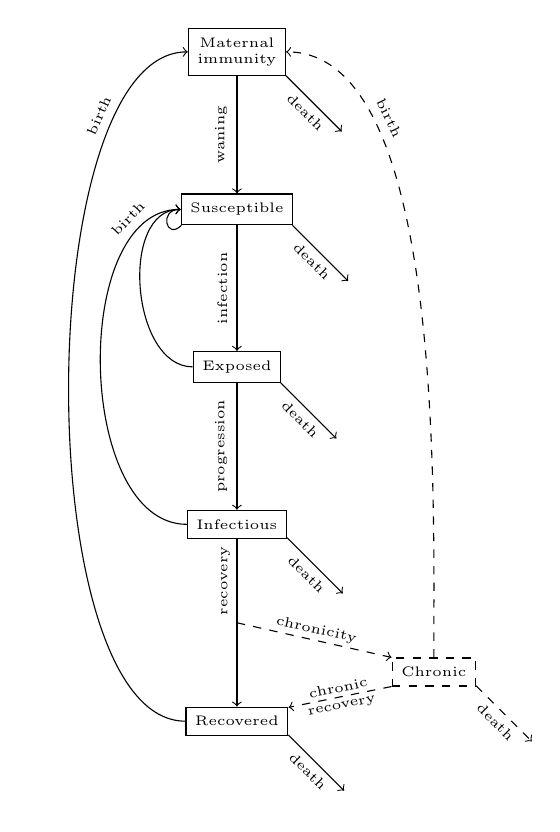
\begin{tikzpicture}[compartment/.style={rectangle, draw},
                    font=\fontsize{5pt}{6}\selectfont]
  % Compartments.
  \node at (0, 8.5) [compartment, align=center, name=MaternalImmunity] {Maternal\\immunity};
  \node at (0, 6.5) [compartment, name=Susceptible] {Susceptible};
  \node at (0, 4.5) [compartment, name=Exposed] {Exposed};
  \node at (0, 2.5) [compartment, name=Infectious] {Infectious};
  \node at (0, 0) [compartment, name=Recovered] {Recovered};
  \node at (2.5, 0.625) [compartment, dashed, name=Chronic] {Chronic};

  % Location for branch from Infectious to Chronic and Recovered.
  \coordinate (recovery) at (0, 1.25);

  % Infection-related processes.
  \draw [->] (MaternalImmunity)
             to node [rotate=90, above] {waning}
             (Susceptible);
  \draw [->] (Susceptible)
             to node [rotate=90, above] {infection}
             (Exposed);
  \draw [->] (Exposed)
             to node [rotate=90, above] {progression}
             (Infectious);
  \draw [  ] (Infectious)
             to node [rotate=90, above, yshift=-1pt] {recovery}
             (recovery);
  \draw [->, dashed] (recovery)
             to node [sloped, above, yshift=-2pt] {chronicity}
             (Chronic.161);
  \draw [->] (recovery)
             to node [] {}
             (Recovered.90);
  \draw [->, dashed] (Chronic.199)
             to node [sloped, align=center] {chronic\\recovery}
             (Recovered.15);
  % \draw [->] (Recovered.195)
  %            to [out=180, in=180] node [left, align=center] {immunity\\waning}
  %            (Susceptible.180);

  % Births
  \draw [->] (Susceptible.196)
             to [out=225, in=180, looseness=3.5] node [] {}
             (Susceptible.180);
  \draw [->] (Exposed.180)
             to [out=180, in=180] node [] {}
             (Susceptible.180);
  \draw [->] (Infectious.180)
             to [out=180, in=180, looseness=0.9] node [sloped, above, pos=0.85] {birth}
             (Susceptible.180);
  \draw [->] (Recovered.180)
             to [out=180, in=180, looseness=0.6] node [sloped, above, pos=0.8] {birth}
             (MaternalImmunity.180);
  \draw [->, dashed] (Chronic.90)
             to [out=90, in=0, looseness=0.65] node [sloped, above, pos=0.75] {birth}
             (MaternalImmunity.0);

  % Deaths
  \draw [->] (MaternalImmunity.334)
             to node [sloped, below, yshift=1pt] {death}
             +(315: 1);
  \draw [->] (Susceptible.344)
             to node [sloped, below, yshift=1pt] {death}
             +(315: 1);
  \draw [->] (Exposed.340)
             to node [sloped, below, yshift=1pt] {death}
             +(315: 1);
  \draw [->] (Infectious.345)
             to node [sloped, below, yshift=1pt] {death}
             +(315: 1);
  \draw [->] (Recovered.345)
             to node [sloped, below, yshift=1pt] {death}
             +(315: 1);
  \draw [->, dashed] (Chronic.342)
             to node [sloped, below, yshift=1pt] {death}
             +(315: 1);
\end{tikzpicture}

%%% Local Variables:
%%% mode: latex
%%% TeX-master: "diagram_standalone"
%%% End:

  \caption{Model diagram.  The dashed box and arrows show the state
    and transitions present in the chronic model but not the acute
    model.}
  \label{fig:diagram}
\end{figure}


The simulations follow a Gillespie algorithm \autocite{gillespie_1977}.
For each buffalo, a list of events and the times they occur is stored.
The next event over the whole population is found and the population
is updated.  The hazards for infection depend on the number of
infectious buffalo in the population and so the times to infection are
updated after each change in the population.  The hazards of the other
events are independent of the state of the population and so the times
to these events are not updated.  This process was repeated from $t =
0$ to $t = t_{\text{max}}$ or until there were $0$ infected (exposed,
infectious, and chronic) buffalo.

When sampling from simple distributions, standard algorithms were used
\autocite{scipy}.  For complex distributions, the event times were
sampled using the inverse transform method \autocite{rubinstein_1981}.

The variables $t$ and $a$ denote time and age, respectively, and are
both in units of years.

\section{Death}

We took the annual survival to be
\begin{equation}
  \Prob\{\text{Survival for $\unit[1]{yr}$}\}
  =
  \begin{cases}
    0.66 & \text{if $a < 1$},
    \\
    0.79 & \text{if $1 \leq a < 3$},
    \\
    0.88 & \text{if $3 \leq a < 12$},
    \\
    0.66 & \text{if $a \geq 12$}.
  \end{cases}
\end{equation}
Assuming that the mortality hazard is constant throughout a year gives
the hazard
\begin{equation}
  h_{\text{mortality}}(a)
  = - \log \Prob\{\text{Survival for $\unit[1]{yr}$}\},
\end{equation}
and the survival
\begin{equation}
  \begin{split}
    S_{\text{mortality}}(a)
    =
    \begin{cases}
      0.66^a
      & \text{if $a < 1$},
      \\
      0.66 \cdot 0.79^{a - 1}
      & \text{if $1 \leq a < 3$},
      \\
      0.66 \cdot 0.79^2 \cdot 0.88^{a - 3}
      & \text{if $3 \leq a < 12$},
      \\
      0.66 \cdot 0.79^2 \cdot 0.88^9 \cdot 0.66^{a - 12}
      & \text{if $a \geq 12$}.
    \end{cases}
  \end{split}
\end{equation}


\section{Birth}

We assumed that females reach reproductive maturity at age $4$ and
that the birth hazard varies at a periodic, triangular-shaped rate in
time:
\begin{equation}
  h_{\text{birth}}(t, a) =
  \begin{cases}
    0 & \text{if $a < 4$},
    \\
    \mu \alpha \max\big(1 - \beta (1 - |1 - 2 \{t - \tau\}|), 0\big)
    & \text{if $a \geq 4$},
  \end{cases}
\end{equation}
with
\begin{equation}
  \alpha =
  \begin{cases}
    1 + c_{\text{v}} \sqrt{3}
    & \text{if $c_{\text{v}} < \frac{1}{\sqrt{3}}$},
    \\
    \frac{3}{2} \left(1 + c_{\text{v}}^2\right)
    & \text{if $c_{\text{v}} \geq \frac{1}{\sqrt{3}}$},
  \end{cases}
\end{equation}
\begin{equation}
  \beta =
  \begin{cases}
    \frac{2 c_{\text{v}} \sqrt{3}}{1 + c_{\text{v}} \sqrt{3}}
    & \text{if $c_{\text{v}} < \frac{1}{\sqrt{3}}$},
    \\
    \frac{3}{4} \left(1 + c_{\text{v}}^2\right)
    & \text{if $c_{\text{v}} \geq \frac{1}{\sqrt{3}}$},
  \end{cases}
\end{equation}
where $\{x\}$ is the fractional part of $x$
(\autoref{fig:birth_hazard}).  The magnitude of the seasonal variation
is captured by the coefficient of variation $c_{\text{v}}$.  The time of year
of the peak birth hazard is $\tau$.  The annual mean $\mu$ was determined
so that the population has asymptotic growth rate $r = 0$.  (See
\autoref{stable_age_distribution}.)

\begin{figure}
  \centering
  \input{birth_hazard.pgf}
  \caption{Model birth hazards for ages 4 years and older.}
  \label{fig:birth_hazard}
\end{figure}

The cumulative hazard for $t$ years, given age $a_0$ at the current
time $t_0$ is
\begin{equation}
  H_{\text{birth}}(t, t_0, a_0) =
  \begin{cases}
    0 & \text{if $a_0 + t < 4$},
    \\
    \mu \left(H_0 + H_1  + H_2\right)
    & \text{if $a_0 + t \geq 4$ and $c_{\text{v}} < \frac{1}{\sqrt{3}}$},
    \\
    \mu \left(H_0 + H_3 + H_4\right)
    & \text{if $a_0 + t \geq 4$ and $c_{\text{v}} \geq \frac{1}{\sqrt{3}}$},
  \end{cases}
\end{equation}
with
\begin{equation}
  \begin{split}
    c &= t_0 + \max(4 - a_0, 0) - \tau,
    \\
    d &= t_0 + t - \tau,
    \\
    H_0 &= \lfloor d \rfloor - \lfloor c \rfloor - 1,
    \\
    H_1 &=
    \begin{cases}
      \frac{1}{2}
      + \alpha \left(\frac{1}{2} - \{c\}\right)
      \left[1 - \beta
        + \beta \left(\frac{1}{2} - \{c\}\right)\right]
      & \text{if $\{c\} < \frac{1}{2}$},
      \\
      \alpha \left(1 - \{c\}\right)
      \left[1 - \beta + \beta \left(1 - \{c\}\right)\right]
      & \text{if $\{c\} \geq \frac{1}{2}$},
    \end{cases}
    \\
    H_2 &=
    \begin{cases}
      \alpha \{d\}\left(1 - \beta \{d\}\right)
      & \text{if $\{d\} < \frac{1}{2}$},
      \\
      \frac{1}{2}
      + \alpha \left(\{d\} - \frac{1}{2}\right)
      \left[1 - \beta
        + \beta \left(\{d\} - \frac{1}{2}\right)\right]
      & \text{if $\{d\} \geq \frac{1}{2}$},
    \end{cases}
    \\
    H_3 &=
    \begin{cases}
      \frac{1}{2} + \alpha \beta \left(\frac{1}{2 \beta} - \{c\}\right)^2
      & \text{if $\{c\} < \frac{1}{2 \beta}$},
      \\
      \frac{1}{2}
      & \text{if $\frac{1}{2 \beta} \leq \{c\} < 1 - \frac{1}{2 \beta}$},
      \\
      \alpha \left(1 - \{c\}\right) \left[1 -
        \beta \left(1 - \{c\}\right)\right]
      & \text{if $\{c\} \geq 1 - \frac{1}{2 \beta}$},
    \end{cases}
    \\
    H_4 &=
    \begin{cases}
      \alpha \{d\} \left[1 - \beta \{d\}\right]
      & \text{if $\{d\} < \frac{1}{2 \beta}$},
      \\
      \frac{1}{2}
      & \text{if $\frac{1}{2 \beta} \leq \{d\} <
        1 - \frac{1}{2 \beta}$},
      \\
      \frac{1}{2}
      + \alpha \beta
      \left[\{d\} - \left(1 - \frac{1}{2 \beta}\right)\right]^2
      & \text{if $\{d\} \geq 1 - \frac{1}{2 \beta}$},
    \end{cases}
  \end{split}
\end{equation}
and $\lfloor x \rfloor$ is the floor function,
i.e.~$\lfloor x \rfloor = x - \{x\}$.
The survival function for $t$ years, given age
$a_0$ at the current time $t_0$ is then
\begin{equation}
  S_{\text{birth}}(t, t_0, a_0) = \exp\left(- H_{\text{birth}}(t, t_0, a_0)\right).
\end{equation}
The probability density function for births time $t$ later, given age
$a_0$ at $t_0$, is
\begin{align}
  f_{\text{birth}}(t, t_0, a_0) =
  h_{\text{birth}}(t_0 + t, a_0 + t)
  S_{\text{birth}}(t, t_0, a_0).
\end{align}

% Multiplying the probability density by $N(t_0, a_0)$, the density of
% females aged $a_0$ at $t_0$, and integrating over $a_0$ gives the
% expected number of births time $t$ later:
% \begin{equation}
%   b(t, t_0) = \int_0^{\infty} f_{\text{birth}}(t, t_0, a_0) N(t_0, a_0) \md a_0.
% \end{equation}
% Binning by month gives the expected number of births in month $m$:
% \begin{align}
%   g(m, t_0) &=
%   \int_0^1 b\left(\frac{m + \mu}{12}, t_0\right) \md \mu
%   & & \text{for $m \in \{0, 1, 2, \ldots\}$}.
% \end{align}

On birth, a newborn is female with probability
$p_{\text{female}} = 0.5$ or otherwise male.


\section{Waning}

The duration of maternal immunity was taken to be a standard gamma
random variable with shape $k_{\text{waning}}$
and mean $\mu_{\text{waning}}$.


\section{Infection}

The infection hazard was taken to be
\begin{equation}
  h_{\text{infection}}(t) = \beta_{\text{acute}} I(t) +
  \beta_{\text{chronic}} C(t),
\end{equation}
where $I(t)$ and $C(t)$ are the total number of infectious and
chronic-carrier buffalo in the herd at time $t$.  Over periods where
$I(t)$ and $C(t)$ are constant, the hazard is constant, which gives an
exponential random variable.


\section{Progression}

The duration of the latent period was taken to be a standard gamma
random variable with shape $k_{\text{progression}}$
and mean $\mu_{\text{progression}}$.


\section{Recovery}

The duration of infection was taken to be a standard gamma random
variable with shape $k_{\text{recovery}}$ and mean
$\mu_{\text{recovery}}$.

On recovery, buffalo become chronic carriers with probability
$p_{\text{chronic}}$ or otherwise are recovered, i.e.~fully cleared
of pathogen.


\section{Chronic recovery}

The duration of the chronic-carrier state was taken to be an
exponential random variable with mean
$\mu_{\text{chronic recovery}}$.


\begin{figure}
  \centering
  \input{distributions.pgf}
  \caption{Hazards and survivals for the model events.}
  \label{fig:distributions}
\end{figure}


\section{Initial conditions}

A sample of size $N$ from the stable age distribution was used to
initialize the population.  (See \autoref{stable_age_distribution}.)
The sex of each buffalo was randomly selected with probability
$p_{\text{female}}$ of being female.

The simulations were started at $t = 0$ with $2$ initial infections
in randomly chosen members of the population.

\cite{hedger_1972}

\cite{medlock_2020}


\section{Stable age distribution}
\label{stable_age_distribution}

The mean rate of female births $B(t)$ follows the Lotka equation
\begin{equation}
  \label{lotka}
  \begin{split}
    B(t) =&
    p_{\text{female}} \bigg[
      \int_0^t B(t - a)
      S_{\text{mortality}}(a)
      h_{\text{birth}}(t, a) \md a
    \\
    & \quad\quad\quad\quad\quad {} +
      \int_0^{\infty} n_0(a)
      \frac{S_{\text{mortality}}(a + t)}{S_{\text{mortality}}(a)}
      h_{\text{birth}}(t, a + t) \md a
    \bigg],
  \end{split}
\end{equation}
where $n_0(a)$ is the density of age $a$ females at time $t = 0$
% Chapter VI, Section 29 on pp.~159--161 of harris_1963
% Chapter 20 on pp.~353--364 of kot_01
\autocite{harris_1963, kot_01}.
% For large $t$, the contribution of the initial cohort---the second
% integral in \eqref{lotka}---becomes negligible, so
% \begin{equation}
%   B(t) =
%   p_{\text{female}} \int_0^t B(t - a)
%   \hat{h}_{\text{birth}}(t, a) \md a
% \end{equation}
% for large $t$,
% where
% \begin{equation}
%   \hat{h}_{\text{birth}}(t, a) =
%   S_{\text{mortality}}(a)
%   h_{\text{birth}}(t, a).
% \end{equation}
% Alternately,
% \begin{equation}
%   B(t)
%   =
%   p_{\text{female}} \int_0^{t}
%   B(u)
%   \hat{h}_{\text{birth}}(t, t - u)
%   \md u.
% \end{equation}
Given $B(t)$, the mean density of females of age $a$ is
\begin{equation}
  n(t, a) =
  \begin{cases}
    B(t - a) S_{\text{mortality}}(a)
    & \text{if $a < t$},
    \\
    n_0(a - t)
    \frac{S_{\text{mortality}}(a)}{S_{\text{mortality}}(a - t)}
    & \text{if $a > t$}.
  \end{cases}
\end{equation}
The mean density of females of age $a$ satisifies the McKendrick--von
Foerster partial differential equation (PDE)
\begin{equation}
  \label{PDE}
  \begin{split}
    \frac{\partial n}{\partial t}(t, a)
    + \frac{\partial n}{\partial a}(t, a)
    &= - h_{\text{death}}(a) n(t, a),
    \\
    n(t, 0) &=
    p_{\text{female}}
    \int_0^{+\infty} h_{\text{birth}}(t, a) n(t, a) \md a,
    \\
    n(0, a) &= n_0(a).
  \end{split}
\end{equation}

Because the birth hazard, $h_{\text{birth}}(t, a)$,
is periodic with period $T = \unit[1]{y}$,
we found the stable age distribution and the asymptotic population growth
rate using Floquet theory \autocite{parker_1992}.
Floquet theory requires the fundamental solution $\Phi(t, a, a')$ for
McKendrick--von Foerster equation \eqref{PDE}, which, for each $a'$,
satisfies the same PDE and birth integral as
$n(t, a)$, but with an initial condition localized to age $a'$:
\begin{equation}
  \label{fundamental_PDE}
  \begin{split}
    \frac{\partial \Phi}{\partial t}(t, a, a')
    + \frac{\partial \Phi}{\partial a}(t, a, a')
    &= - h_{\text{death}}(a) \Phi(t, a, a'),
    \\
    \Phi(t, 0, a') &=
    p_{\text{female}}
    \int_0^{+\infty} h_{\text{birth}}(t, a) \Phi(t, a, a') \md a,
    \\
    \Phi(0, a, a') &= \delta(a - a'),
  \end{split}
\end{equation}
where $\delta(x)$ is the Dirac delta.
To solve this numerically, we used the
Crank--Nicolson method on characteristics and the composite trapezoid
rule for the birth integral \autocite{milner_1992}.  Given the time
step $\Delta t$,
let $a_i = i \Delta t$
and $a'_j = j \Delta t$
for $i, j \in \{0, 1, 2, \ldots, I - 1\}$;
$t^k = k \Delta t$
for $k \in \{0, 1, \ldots, K - 1\}$;
and $\Phi_{i, j}^k \approx \Phi(t^k, a_i, a'_j)$.
For each $j$ and each $k \geq 1$, the Crank--Nicolson method on
characteristics is
\begin{equation}
  \label{CN_step}
  \frac{\Phi_{i, j}^k - \Phi_{i - 1, j}^{k - 1}}{\Delta t}
  = - h_{\text{death}}(a_{i - 1 / 2})
  \frac{\Phi_{i, j}^k + \Phi_{i - 1, j}^{k - 1}}{2},
\end{equation}
or
\begin{equation}
  \Phi_{i, j}^k
  = \frac{1 - C_{i - 1 / 2}}{1 + C_{i - 1 / 2}}
  \Phi_{i - 1, j}^{k - 1},
\end{equation}
with
\begin{equation}
  C_{i - 1 / 2}
  = \frac{h_{\text{death}}(a_{i - 1 / 2}) \Delta t}{2},
\end{equation}
for $i \in \{1, 2, \ldots, I - 2\}$.  For $i = I - 1$,
a term was added to prevent buffaloes from aging out of this
last age group:
\begin{equation}
  \Phi_{I - 1, j}^k
  = \frac{1 - C_{I - 3 / 2}}{1 + C_{I - 3 / 2}}
  \Phi_{I - 2, j}^{k - 1}
  + \frac{1 - C_{I - 1}}{1 + C_{I - 1}}
  \Phi_{I - 1, j}^{k - 1},
\end{equation}
with
\begin{equation}
  C_{I - 1}
  = \frac{h_{\text{death}}(a_{I - 1}) \Delta t}{2}.
\end{equation}
For $i = 0$, the birth integral is given by the composite trapezoid rule,
\begin{equation}
  \label{birth_step}
  \Phi_{0, j}^k =
  \frac{p_{\text{female}} \Delta t}{2}
  \sum_{i = 1}^{I - 1}
  \left[h_{\text{birth}}(t^k, a_i) \Phi_{i, j}^k +
    h_{\text{birth}}(t^k, a_{i - 1}) \Phi_{i - 1, j}^k\right].
\end{equation}
The initial condition is
\begin{equation}
  \Phi_{i, j}^0 =
  \begin{cases}
    1 & \text{if $i = j$}, \\
    0 & \text{otherwise}.
  \end{cases}
\end{equation}
Considering $\mat{\Phi}^k = [\Phi_{i, j}^k]$ as a matrix that
evolves in time, the method is easily implemented with matrix algebra:
the Crank--Nicolson step \eqref{CN_step} is
\begin{equation}
  \mat{\Phi}^k = \mat{M} \mat{\Phi}^{k - 1},
\end{equation}
with the matrix $\mat{M} = [M_{i, j}]$ where
\begin{equation}
  M_{i, j} =
  \begin{cases}
    \frac{1 - C_{i - 1 / 2}}{1 + C_{i - 1 / 2}}
    & \text{if $i = j + 1$}, \\
    \frac{1 - C_{I - 1}}{1 + C_{I - 1}} & \text{if $i = j = I - 1$}, \\
    0 & \text{otherwise};
  \end{cases}
\end{equation}
the birth integral \eqref{birth_step} is then
\begin{equation}
  \mat{\Phi}_0^k = \vec{v} \mat{\Phi}^k,
\end{equation}
with the vector $\vec{v} = [v_i]$ where
\begin{equation}
  v_i =
  \begin{cases}
    \frac{p_{\text{female}} \Delta t}{2}
    & \text{if $i = 0$ or $i = I - 1$}, \\
    p_{\text{female}} \Delta t
    & \text{otherwise};
  \end{cases}
\end{equation}
and the initial condition is
\begin{equation}
  \mat{\Phi}^0 = \mat{I},
\end{equation}
where $\mat{I}$ is the $I \times I$ identity matrix.

Using this numerical scheme, we solved for the monodromy matrix, the
fundamental solution after one period:
\begin{equation}
  \mat{\Psi} = [\Psi_{i, j}] \approx [\Phi(T, a_i, a'_j)].
\end{equation}
The monodromy matrix projects the population forward at by one period,
\begin{equation}
  \vec{n}(T) = \mat{\Psi} \vec{n}(0),
\end{equation}
where $\vec{n}(t) = [n(t, a_i)]$.
Using the monodromy operator to repeatedly project the population
forward gives
\begin{equation}
  \vec{n}(K T)
  = \mat{\Psi}^K \vec{n}(0)
  \to \rho_0^K \vec{w}_0
  = \me^{r K T} \vec{w}_0
\end{equation}
as $K \to \infty$,
where $\rho_0$ is the dominant eigenvalue, i.e. the eigenvalue with
largest magnitude, of $\mat{\Psi}$;
the corresponding right eigenvector $\vec{w}_0$ is the stable age
distribution; and
\begin{equation}
  r = \frac{1}{T} \log \rho_0
\end{equation}
is the asymptotic population growth rate.

We numerically computed the population growth rate and stable age
distribution by using age and time steps $\Delta t = 0.01$,
maximum age $a_{\text{max}} = 35$
(probability of survival
$S_{\text{mortality}}(35) \approx 10^{-5}$),
finding the monodromy matrix by numerically solving
\eqref{fundamental_PDE} from $t = 0$ to $T$, and
then finding its dominant eigenvalue and corresponding eigenvector.
We then used a root-finding algorithm to find the value of the mean
birth hazard $\mu \approx 0.9379$ that gave growth rate $r = 0$.
Halving the age step to $\Delta a = 0.005$
gave a relative error for $\mu$ of $7 \times 10^{-4}$
and doubling the maximum age to $a_{\text{max}} = 70$
gave a relative error of $5 \times 10^{-6}$.
These computations were done in Python \autocite{python} using the
NumPy \autocite{numpy} and SciPy \autocite{scipy} libraries.


\begin{figure}
  \centering
  \input{stable_age_distribution.pgf}
  \caption{TODO: Write caption.
    This is on 01 July and the birth peak is 01 January.
    Reference this figure in the text.}
  \label{fig:stable_age_distribution}
\end{figure}


\printbibliography


\newpage
\appendix
\section*{Supplemental Results Figures}
% These figure numbers will start after the previous appendix.
% I.e. if the previous was Appendix S3, these will be Figure S4,
% Figure S5, ...
\setcounter{figure}{\value{chapter}}
\renewcommand{\thefigure}{\appendixlabel\arabic{figure}}
\renewcommand{\HyperDestNameFilter}[1]{chapter-#1}


\begin{figure}
  \centering
  \includegraphics{../population_sizes}
  \caption{The sensitivity of extinction time of FMDV to buffalo
    population size.
    For each model and each SAT, the model was simulated for 1000 runs
    at population sizes 100, 200, 300, 400, 500, 600, 700, 800, 900,
    1000 (baseline, dotted vertical lines), 2000, 3000, 4000, and
    5000.
    The other parameters were fixed at their baseline values.
    The top and middle rows of graphs show the distribution of
    FMDV extinction times for the model with only acute transmission
    and the model with both acute and chronic transmission,
    respectively.
    The bottom row shows the proportion of simulations where FMDV
    persisted in the buffalo population for the whole simulated
    10-year period for the model with both acute and chronic
    transmission.}
\end{figure}

\begin{figure}
  \centering
  \includegraphics{../birth_seasonality}
  \caption{The sensitivity of extinction time to birth seasonality.
    For each model and each SAT, the model was simulated for
    1000 runs at 0, 0.5, 1 (baseline, dotted vertical lines), 1.5, and
    2 times the baseline birth seasonal coefficient of variation of
    0.613.
    The other parameters were fixed at their baseline values.
    The top and middle rows of graphs show the distribution of
    FMDV extinction times for the model with only acute transmission
    and the model with both acute and chronic transmission,
    respectively.
    The bottom row shows the proportion of simulations where FMDV
    persisted in the buffalo population for the whole simulated
    10-year period with both acute and chronic transmission.}
\end{figure}

\begin{figure}
  \centering
  \includegraphics{../samples_sensitivity_acute}
  \caption{The sensitivity of FMDV extinction time to model
    parameters, for the model with only acute transmission.
    The sensitivity is measured by the partial rank correlation
    coefficient (PRCC) \autocite{blower_1994}.
    The model was simulated with each of 20,000 samples from the
    posterior distributions of the parameters
    (Fig.~2; Tables S2, S3).}
\end{figure}


\end{document}
